\documentclass[aspectratio=169,11pt]{beamer}

\IfFileExists{beamerthememetropolis.sty}{%
  \usetheme[numbering=fraction,progressbar=frametitle]{metropolis}
}{%
  \usetheme{CambridgeUS}
  \usecolortheme{dolphin}
}

\usepackage{iftex}
\ifXeTeX
  \usepackage{fontspec}
  \usepackage{xeCJK}
  \usepackage{unicode-math}
  \IfFontExistsTF{Times New Roman}{\setmainfont{Times New Roman}}{\setmainfont{TeX Gyre Termes}}
  \IfFontExistsTF{STIX Two Math}{\setmathfont{STIX Two Math}}{}
  \IfFontExistsTF{PingFang SC}{%
    \setCJKmainfont{PingFang SC}
  }{%
    \IfFontExistsTF{Songti SC}{\setCJKmainfont{Songti SC}}{\setCJKmainfont{STFangsong}}
  }
\else
  \usepackage[T1]{fontenc}
  \usepackage[utf8]{inputenc}
  \usepackage{lmodern}
\fi

\usepackage{booktabs}
\usepackage{tabularx}
\usepackage{array}
\usepackage{graphicx}
\usepackage{amsmath}
\usepackage{adjustbox}

\setbeamertemplate{navigation symbols}{}
\setbeamertemplate{footline}[frame number]

\definecolor{zjublue}{RGB}{28,72,116}
\definecolor{ink}{RGB}{45,45,45}
\definecolor{softblue}{RGB}{232,240,248}
\definecolor{softgray}{RGB}{245,246,248}
\definecolor{softgreen}{RGB}{232,244,235}
\definecolor{softred}{RGB}{248,235,233}

\setbeamercolor{frametitle}{fg=white,bg=black!78}
\setbeamercolor{title}{fg=zjublue}
\setbeamercolor{structure}{fg=zjublue}
\setbeamercolor{normal text}{fg=ink}
\setbeamercolor{boxblue}{bg=softblue,fg=ink}
\setbeamercolor{boxgray}{bg=softgray,fg=ink}
\setbeamercolor{boxgreen}{bg=softgreen,fg=ink}
\setbeamercolor{boxred}{bg=softred,fg=ink}
\setbeamerfont{frametitle}{size=\Large,series=\bfseries}
\setbeamerfont{title}{size=\LARGE,series=\bfseries}
\setbeamersize{text margin left=0.70cm,text margin right=0.70cm}
\renewcommand{\arraystretch}{1.13}
\graphicspath{{figures/}}

\newcommand{\tightitem}{\setlength\itemsep{0.25em}}
\newcommand{\plainbox}[2]{%
  \begin{beamercolorbox}[rounded=true,sep=0.48em,wd=\textwidth]{#1}
    #2
  \end{beamercolorbox}
}

\title{When Do Critical-Mineral Export Controls Bind?}
\subtitle{China's Licensing-Based Controls and Heterogeneous Trade Responses}
\author{Mario Diez Mart\'inez}
\institute{Master Program in Chinese Economy\\Supervisor: 杜立民}
\date{}

\begin{document}

% Slide 1
\begin{frame}[plain]
  \vspace{0.60cm}
  {\usebeamerfont{title}\usebeamercolor[fg]{title}
  When Do Critical-Mineral\\Export Controls Bind?\par}
  \vspace{0.28cm}
  {\large China's Licensing-Based Controls and Heterogeneous Trade Responses\par}
  \vfill
  {\large Mario Diez Mart\'inez\par}
  \vspace{0.16cm}
  {Master Program in Chinese Economy\par}
  {Supervisor: 杜立民\par}
\end{frame}

% Slide 2
\begin{frame}{Research Background}
  \begin{columns}[T,totalwidth=\textwidth]
    \begin{column}{0.50\textwidth}
      \normalsize
      \begin{itemize}
        \tightitem
        \item Critical minerals are inputs for chips, batteries, defense, and energy equipment.
        \item China is central in many refining and processing stages.
        \item Recent controls use export licensing, not automatic export bans.
        \item The outcome is observed trade adjustment, not the legal rule alone.
      \end{itemize}
    \end{column}
    \begin{column}{0.46\textwidth}
      \plainbox{boxblue}{%
        \textbf{Research question}\\[0.12cm]
        Why do formally similar Chinese export-licensing controls generate different trade and price disruptions across critical minerals?
      }
    \end{column}
  \end{columns}
\end{frame}

% Slide 3
\begin{frame}{Literature Review}
  \footnotesize
  \begin{columns}[T,totalwidth=\textwidth]
    \begin{column}{0.49\textwidth}
      \textbf{Economic statecraft}\\
      Chokepoints and sanctions channels.\\
      {\scriptsize (Farrell and Newman, 2019; Egger et al., 2024).}

      \vspace{0.18cm}
      \textbf{Export licensing}\\
      Legal treatment, product language, and dates.\\
      {\scriptsize (PRC Export Control Law, 2020; SCIO, 2021; State Council, 2024; MOFCOM/GAC, 2023--2025).}
    \end{column}
    \begin{column}{0.49\textwidth}
      \textbf{Critical minerals}\\
      Concentration matters, but HS scope and substitution differ.\\
      {\scriptsize (IEA, 2025; OECD, 2026).}

      \vspace{0.18cm}
      \textbf{Trade methods}\\
      PPML, triple difference, event timing, and cautious inference.\\
      {\scriptsize (Santos Silva and Tenreyro, 2006; Fally, 2015; Olden and Moen, 2022; Conley and Taber, 2011).}
    \end{column}
  \end{columns}

  \vspace{0.08cm}
  \plainbox{boxblue}{%
    \small Gap: recent Chinese critical-mineral licensing waves have not been linked cleanly to product-source monthly trade evidence, HS observability, and switching-versus-compression margins.
  }
\end{frame}

% Slide 4
\begin{frame}{Empirical Design: Data Sources}
  \small
  \begin{columns}[T,totalwidth=\textwidth]
    \begin{column}{0.49\textwidth}
      \plainbox{boxblue}{%
        \textbf{Main trade panel}
        \begin{itemize}
          \tightitem
          \item UN Comtrade monthly bilateral imports.
          \item Current panel: 53 reporters, 10 HS products, Jan. 2019--Mar. 2026.
          \item Variables: \(M_{ipst}\), China/RoW imports, total imports, supplier count, supplier HHI.
        \end{itemize}
      }
    \end{column}
    \begin{column}{0.49\textwidth}
      \plainbox{boxgray}{%
        \textbf{Auxiliary data}
        \begin{itemize}
          \tightitem
          \item Policy: Chinese laws and MOFCOM/GAC notices.
          \item Prices: matched domestic and international benchmarks.
          \item Demand: semiconductors, batteries, steel, lead-acid batteries.
          \item Structure/geography: USGS/IEA concentration and CEPII distance.
        \end{itemize}
      }
    \end{column}
  \end{columns}

  \vspace{0.12cm}
  {\footnotesize Observation unit: importer \(i\) \(\times\) HS product \(p\) \(\times\) source \(s\) \(\times\) month \(t\). Example: Germany, HS 282580, China, Nov. 2024, import value in USD.}
\end{frame}

% Slide 5
\begin{frame}{Empirical Design: Product Waves}
  \footnotesize
  \begingroup
  \setlength{\tabcolsep}{3pt}
  \renewcommand{\arraystretch}{1.02}
  \begin{tabularx}{\textwidth}{>{\raggedright\arraybackslash\bfseries}p{0.17\textwidth}>{\raggedright\arraybackslash}p{0.43\textwidth}>{\raggedright\arraybackslash}X}
    \toprule
    Wave or role & HS products & Current role \\
    \midrule
    Aug. 2023 Ga/Ge & Ga/Ge bundle HS 811292; GeO2/ZrO2 HS 282560 & complete; partial/bundled HS match \\
    Dec. 2023 C & natural graphite HS 2504; artificial/colloidal graphite HS 3801 & HS 3801 is partially treated, diagnostic only \\
    Sept. 2024 Sb & Sb metal HS 8110; Sb ores HS 261710; Sb oxides HS 282580 & complete; scope and trade regularity differ \\
    Feb. 2025 W/Bi etc. & Bi HS 8106; APT/tungstates HS 284180; W HS 8101; etc. & expansion sample after coverage audit \\
    Candidate donors & alumina HS 2818; Mn HS 8111; inorganic acids HS 2811; Mo/metal-family candidates; etc. & current estimates use 2818, 8111, 2811 \\
    \bottomrule
  \end{tabularx}
  \endgroup

  \vspace{0.05cm}
  \plainbox{boxgray}{%
    \scriptsize Expanded donor candidates are fixed in the data plan, but final use depends on policy-status, coverage, trade-regularity, and suitability checks.
  }
\end{frame}

% Slide 6
\begin{frame}{Empirical Design: Model}
  \vspace{-0.12cm}
  \[
  \mathbb{E}[M_{ipst}\mid X_{ipst}] =
  \exp\left[
  \beta (Treated_p \times China_s \times Post_{pt})
  + \alpha_{ips}+\delta_{it}+\lambda_{pt}+\mu_{st}
  \right].
  \]

  \vspace{-0.06cm}
  \begin{columns}[T,totalwidth=\textwidth]
    \begin{column}{0.49\textwidth}
      \small
      \textbf{Why PPML?}
      {\scriptsize (Santos Silva and Tenreyro, 2006)}
      \begin{itemize}
        \tightitem
        \item Keeps zero trade flows.
        \item Fits trade values with very different scales.
        \item Avoids log-OLS problems under heteroskedasticity.
        \item Gives proportional effects.
      \end{itemize}

      \vspace{0.08cm}
      \(\text{Effect}=100\times(e^\beta-1)\).
    \end{column}
    \begin{column}{0.49\textwidth}
      \small
      \textbf{Treatment term}
      \begin{itemize}
        \tightitem
        \item \(M_{ipst}\): import value.
        \item \(Treated_p\): HS product in a policy wave.
        \item \(China_s\): source is China.
        \item \(Post_{pt}\): expected import-effect month onward.
        \item \(\beta\): relative China-source post-policy change.
      \end{itemize}
    \end{column}
  \end{columns}

  \vspace{0.08cm}
  {\scriptsize Fixed effects: \(\alpha_{ips}\) baseline sourcing; \(\delta_{it}\) importer-month shocks; \(\lambda_{pt}\) product-month shocks; \(\mu_{st}\) China/RoW source-month shocks.}
\end{frame}

% Slide 7
\begin{frame}{Empirical Design: Diagnostics}
  \small
  \begin{columns}[T,totalwidth=\textwidth]
    \begin{column}{0.48\textwidth}
      \textbf{Hypotheses}
      \begin{itemize}
        \tightitem
        \item \textbf{H1 Trade-binding:} \(\beta<0\) in the source-contrast PPML.
        \item \textbf{H2 Timing:} no systematic pre-policy event-study decline.
        \item \textbf{H3 Adjustment:} switching if China falls and RoW rises; compression if total imports fall.
      \end{itemize}
    \end{column}
    \begin{column}{0.48\textwidth}
      \textbf{Interpretation checks}
      \begin{itemize}
        \tightitem
        \item Product scope: clean, partial, bundled, or sparse HS code.
        \item Price wedge: secondary scarcity or segmentation diagnostic.
        \item Exposure/access: mechanism split for H3.
        \item Inference: reporter \(p\)-values are conditional diagnostics.
      \end{itemize}
    \end{column}
  \end{columns}

  \vspace{0.16cm}
  \plainbox{boxblue}{%
    \small Strong evidence requires H1 plus timing support. H3 then tells whether the response is source switching or import compression.
  }
\end{frame}

% Slide 8
\begin{frame}{Preliminary Results}
  \scriptsize
  \begin{tabularx}{\textwidth}{>{\raggedright\arraybackslash}p{0.33\textwidth}>{\raggedright\arraybackslash}p{0.10\textwidth}>{\raggedleft\arraybackslash}p{0.18\textwidth}>{\raggedleft\arraybackslash}p{0.13\textwidth}>{\raggedright\arraybackslash}X}
    \toprule
    Product or sample & HS & Effect & \(p\)-value & Pre-period diagnostic \\
    \midrule
    Natural graphite & 2504 & \(-30.4\%\) & 0.107 & Rejected \\
    Gallium/germanium bundle & 811292 & \(+19.3\%\) & 0.365 & Rejected \\
    GeO2/ZrO2 & 282560 & \(+17.5\%\) & 0.271 & Not rejected \\
    Antimony metal & 8110 & \(-86.8\%\) & \(<0.001\) & Rejected \\
    Antimony ores/concentrates & 261710 & \(-98.9\%\) & 0.003 & Rejected \\
    Antimony oxides & 282580 & \(-81.5\%\) & 0.002 & Not rejected \\
    Antimony oxides, high exposure/access & 282580 & \(-87.4\%\) & \(<0.001\) & Not rejected \\
    \bottomrule
  \end{tabularx}

  \vspace{0.08cm}
  {\scriptsize Each row estimates the Slide 6 PPML model for one treated HS product against HS 2818, HS 8111, and HS 2811 as current controls. The \(p\)-value is reporter-clustered and conditional. The pre-period diagnostic is a joint test of pre-policy event-time coefficients. High exposure/access means pre-policy China dependence plus observed RoW sourcing.}
\end{frame}

% Slide 9
\begin{frame}{Preliminary Results: HS 282580}
  \begin{columns}[T,totalwidth=\textwidth]
    \begin{column}{0.62\textwidth}
      \centering
      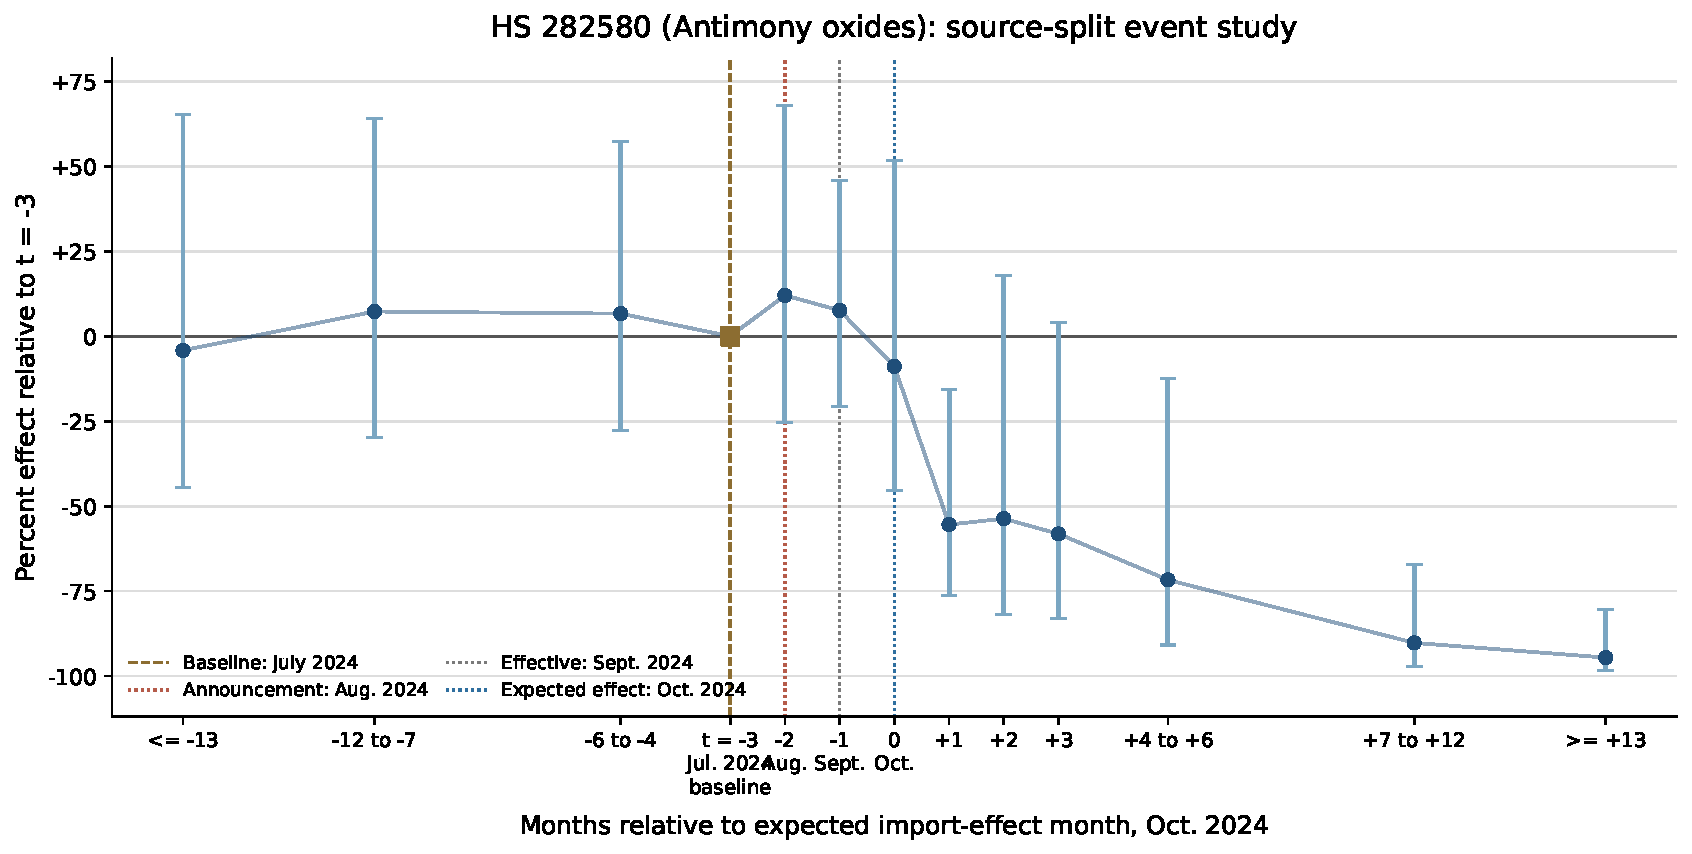
\includegraphics[width=\textwidth,height=0.52\textheight,keepaspectratio]{hs282580_eventstudy_slides.pdf}
    \end{column}
    \begin{column}{0.34\textwidth}
      \normalsize
      \begin{itemize}
        \tightitem
        \item Product: antimony oxides.
        \item Expected import-effect month: Oct. 2024.
        \item Main effect: \(-81.5\%\), \(p=0.002\).
        \item Pre-period diagnostic: joint event-study test, \(p=0.680\).
      \end{itemize}
    \end{column}
  \end{columns}

  \vspace{0.14cm}
  \plainbox{boxblue}{%
    \small The pre-period test checks whether pre-policy event coefficients are jointly zero. Here it is not rejected; the result remains feasibility evidence, not proof of license denial or welfare loss.
  }
\end{frame}

% Slide 10
\begin{frame}{References}
  \small
  \begin{itemize}
    \tightitem
    \item \textbf{Economic statecraft:} Farrell and Newman (2019) on chokepoints; Egger, Syropoulos, and Yotov (2024) on sanctions and quantification.
    \item \textbf{Legal coding:} PRC Export Control Law, SCIO white paper, 2024 Dual-Use Regulation, and MOFCOM/GAC mineral-control notices.
    \item \textbf{Critical-mineral context:} IEA (2025) on supply concentration; OECD (2026) on export restrictions for critical raw materials.
    \item \textbf{Empirical method:} Santos Silva and Tenreyro (2006) for PPML; Fally (2015) for fixed effects; Olden and Moen (2022) for triple difference.
    \item \textbf{Inference and timing:} Conley and Taber (2011), Ferman and Pinto (2019), MacKinnon and Webb (2018), and Roth (2022).
  \end{itemize}
\end{frame}

\appendix

% Backup slide 1
\begin{frame}[noframenumbering]{Backup: Price Wedge Diagnostic}
  \[
  \log P_{rpt} =
  \alpha_{rp}+\lambda_{pt}
  + \delta (International_r \times Post_{pt})
  + \epsilon_{rpt}.
  \]

  \vspace{0.05cm}
  \small
  \begin{itemize}
    \tightitem
    \item \(P_{rpt}\): benchmark price for region \(r\), product \(p\), month \(t\).
    \item \(International_r\): benchmark is international rather than Chinese domestic.
    \item \(Post_{pt}\): expected import-effect month onward.
    \item \(\delta\): post-policy international-relative-to-domestic price wedge.
    \item Use only when grade, unit, location, currency, and tax basis match.
  \end{itemize}

  \vspace{0.08cm}
  \plainbox{boxgray}{%
    \small This is a descriptive diagnostic unless final matched price data support a stronger design.
  }
\end{frame}

% Backup slide 2
\begin{frame}[noframenumbering]{Backup: Exposure and Access}
  \small
  \plainbox{boxblue}{%
    \small Theoretical role: licensing creates an unobserved wedge. H3 asks whether exposed importers with outside suppliers switch sources rather than compress total imports.
  }

  \vspace{0.14cm}
  \begin{itemize}
    \tightitem
    \item \(E_{ip}\): importer \(i\)'s pre-policy dependence on China for product \(p\).
    \item \(O_{ip}\): importer \(i\)'s pre-policy rest-of-world sourcing frequency for product \(p\).
    \item \(A_{ip}=E_{ip}\times O_{ip}\): compact exposure-and-access proxy.
  \end{itemize}

  \vspace{0.18cm}
  \plainbox{boxgray}{%
    \small Test: split importers by \(A_{ip}\), re-estimate the same source-contrast PPML, and compare China, RoW, and total-import margins. \(A_{ip}\) is a proxy, not proof of true substitute availability.
  }
\end{frame}

\end{document}
